\chapter{Anonimato e Privacy}

Prima di analizzare le tecniche di anonimato all'interno della blockchain, è necessario definire con precisione cosa significhi questo termine in ambito informatico. Generalmente, il concetto si presta a due interpretazioni principali:
\begin{itemize}
    \item Interagire \textbf{senza utilizzare il proprio vero nome} (ma impiegando un alias testuale o numerico).
    \item Interagire \textbf{senza rivelare alcuna identità} o traccia riconducibile al singolo individuo.
\end{itemize}

Nel caso di Bitcoin, la prima interpretazione è chiaramente soddisfatta, poiché gli utenti utilizzano gli hash delle proprie chiavi pubbliche (gli indirizzi) come identità. Tuttavia, la seconda interpretazione non lo è. Questa distinzione ci porta a definire il sistema Bitcoin non come anonimo, bensì come \textbf{pseudo-anonimo}. 

Lo pseudo-anonimato, da solo, non è sufficiente a garantire la privacy su un registro pubblico. In crittografia, il vero anonimato si definisce come la somma di due proprietà: \textbf{Pseudo-anonimato + Unlinkability} (Non-collegabilità). 
L'\textit{unlinkability} è la proprietà per cui differenti interazioni dello stesso utente non possono essere correlate tra loro dal sistema o da un osservatore esterno. Per ottenere un'effettiva privacy in Bitcoin, dovrebbero verificarsi tre condizioni di \textit{unlinkability}:
\begin{itemize}
    \item Deve essere computazionalmente difficile ricollegare indirizzi diversi allo stesso utente reale.
    \item Deve essere difficile ricollegare transazioni diverse al medesimo utente.
    \item Deve essere difficile ricollegare il mittente di un pagamento al suo effettivo destinatario.
\end{itemize}

Mentre per i primi due casi è possibile adottare euristiche e buone pratiche (come generare un nuovo indirizzo per ogni transazione), il terzo caso è intrinsecamente violato dall'architettura base del protocollo: analizzando una singola transazione standard, il collegamento logico tra l'input (mittente) e l'output (destinatario) è pubblico e palese. Offuscare questo legame diventa fattibile solo se consideriamo la transazione non come un singolo evento isolato, ma come un flusso all'interno di un grafo di transazioni complesse.

Poiché garantire una completa \textit{unlinkability} sull'intero network è impossibile, l'obiettivo crittografico è quello di rendere anonima almeno una porzione delle transazioni, nascondendole all'interno di un \textbf{Anonymity Set} (Insieme di Anonimato). L'efficacia di queste tecniche dipenderà direttamente dal \textit{Threat Model}: dobbiamo cioè stabilire a priori \textbf{chi è l'attaccante e quali sono le sue capacità} di analisi della rete.

\section{Perché vogliamo l'anonimato?}
Poiché la blockchain è un \textit{ledger} (registro) completamente pubblico, l'assenza di anonimato comporta enormi criticità. Nel sistema bancario tradizionale, il registro delle transazioni è privato e custodito da un ente fiduciario; nessuno, tranne le autorità competenti, può accedere allo storico finanziario di un cittadino. Al contrario, in Bitcoin chiunque può ispezionare il registro, calcolare il saldo di una certa identità pseudo-anonima, e tracciarne ogni singolo movimento in entrata e in uscita.

Questa trasparenza estrema espone gli utenti a veri e propri tracciamenti finanziari. Se l'identità reale di un utente viene associata al suo indirizzo, è possibile per chiunque compiere azioni di spionaggio (ad esempio, un'azienda potrebbe monitorare i fornitori e i volumi d'affari di un competitor). 

Spesso si associa erroneamente la richiesta di anonimato finanziario ad attività illecite (acquisto di beni illegali, riciclaggio, evasione fiscale). Sebbene la tecnologia possa essere abusata, il diritto alla privacy finanziaria è un'esigenza legittima per proteggersi da sorveglianza di massa e attacchi mirati. Inoltre, anche i fondi di provenienza illecita, per poter essere utilizzati nell'economia reale, prima o poi devono transitare attraverso un punto di conversione in valuta \textit{fiat} (\textit{exchange} con procedure KYC/AML), rendendo di fatto possibile il tracciamento da parte delle forze dell'ordine. La neutralità della tecnologia crittografica è simile a quella della rete Tor: uno strumento \textit{agnostico} che fornisce privacy a prescindere dall'intento etico o meno dell'utente finale.

\subsection{Anonymous e-cash e Blind Signatures}
Una delle primissime e più eleganti soluzioni per i pagamenti digitali anonimi fu proposta dal crittografo David Chaum nel 1982. L'idea alla base di \textit{e-cash} era quella di consentire pagamenti digitali mantenendo una banca come autorità centrale fidata per la contabilità, ma impedendole matematicamente di tracciare le abitudini di spesa dei propri clienti.

Il protocollo si basa sul concetto crittografico delle \textbf{Blind Signatures} (Firme Cieche) e si articola in tre fasi:

\begin{itemize}
    \item \textbf{1. Fase di Prelievo (\textit{Withdrawal}):} L'utente Alice genera un numero seriale casuale $S$, che rappresenterà univocamente la moneta elettronica. Per nasconderlo alla banca, Alice applica una funzione di \textit{blinding} (mascheramento) utilizzando un fattore casuale $r$, ottenendo un \textit{commitment} $M = f(S, r)$. Alice invia $M$ alla banca richiedendo un prelievo.
    La banca autentica Alice, verifica i fondi sul suo conto e li detrae. Successivamente, la banca applica la propria firma digitale sul \textit{commitment} cieco, generando $\text{Sign}_{\text{bank}}(M)$, e la restituisce ad Alice. La banca ha firmato la moneta senza averne mai visto il vero numero seriale $S$.
    
    \item \textbf{2. Fase di Unblinding:} Ricevuta la firma cieca, Alice utilizza il fattore $r$ per rimuovere il mascheramento matematico applicato in precedenza. Grazie alle proprietà omomorfiche delle \textit{blind signatures}, questa operazione restituisce una firma della banca perfettamente valida applicata direttamente al seriale in chiaro: $\text{Sign}_{\text{bank}}(S)$.
    
    \item \textbf{3. Fase di Deposito (\textit{Deposit}):} Alice desidera acquistare un bene da Bob e gli consegna la moneta $(S, \text{Sign}_{\text{bank}}(S))$. Bob verifica crittograficamente la firma usando la chiave pubblica della banca e, per concludere la transazione, invia la moneta alla banca per farsi accreditare l'importo. La banca riceve il seriale $S$, verifica la propria firma e controlla nel suo database che $S$ non sia mai stato speso prima (prevenendo il \textit{Double Spending}). Se $S$ è nuovo, la banca accredita i fondi sul conto di Bob.
\end{itemize}

\textbf{La garanzia di Anonimato:} Durante il deposito, la banca vede il numero seriale $S$ per la prima volta. Non ha alcun modo crittografico per collegare questo seriale $S$ al \textit{commitment} $M$ che aveva firmato ad Alice durante la fase di prelievo. Di conseguenza, pur mantenendo il controllo assoluto contro la doppia spesa, l'autorità centrale non può assolutamente sapere chi ha pagato Bob, garantendo così un anonimato totale e matematicamente provato per il pagatore.

\begin{figure}[H]
    \centering
    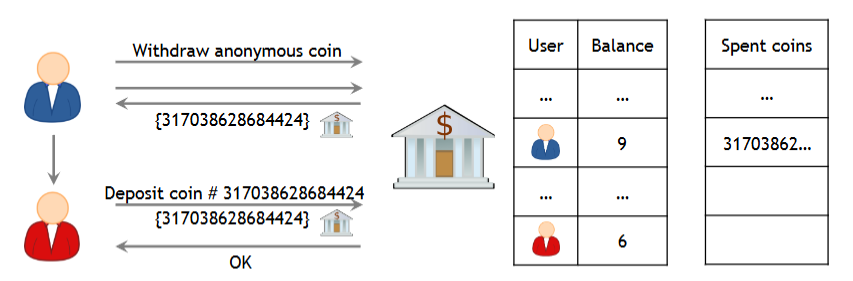
\includegraphics[width=0.9\linewidth]{Images/capitolo_4/transazione_blind.png}
\end{figure}
Naturalmente, per garantire tale anonimato abbiamo bisogno di spese unitarie o, al più, un numero limitato di quantità "prestabilite" in maniera tale che la banca non possa fare linking mediante la cifra spesa. Si presuppone chiaramente che il sistema sia utilizzato da più persone poiché altrimenti il link risulta banale.

Il vero e proprio problema è il fatto che i protocolli interattivi con la banca sono complicati da gestire e da decentralizzare soprattutto.

\subsection{Anonimato grazie a nuovi indirizzi}
Supponiamo che A voglia ottenere il massimo anonimato dal sistema blockchain e che, intuitivamente, decide di usare sempre indirizzi diversi per ogni transazione. 

Siamo adesso nella situazione in cui A voglia comprare un oggetto e, per farlo, necessita di un certo numero di monete che sono, quindi, dentro tanti UTXO diversi che hanno una firma diversa.
\begin{figure}[H]
    \centering
    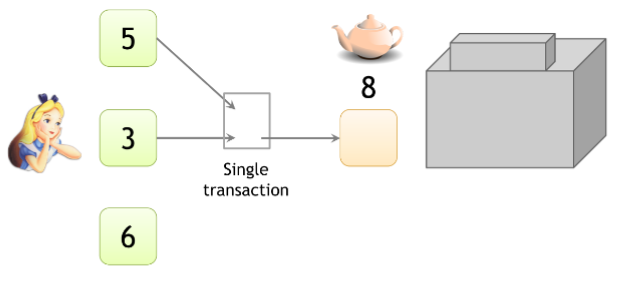
\includegraphics[width=0.6\linewidth]{Images/capitolo_4/tegliera.png}
\end{figure}
Poiché un attaccante vede una transazione verso una certa autorità, \footnote{Vedremo dopo come questa cosa venga capita} questo vede prima la transazione di compattazione degli uTXO e, quindi, riesce a collegare che quei due UTXO appartenevano alla stessa entità. Non solo, se il pagamento non è per intero, allora è necessario dare il resto che, quindi, apparterrà alla stessa entità del pagamento.

Tramite queste intuizioni, possiamo tracciare un grafo di questo tipo:
\begin{figure}[H]
    \centering
    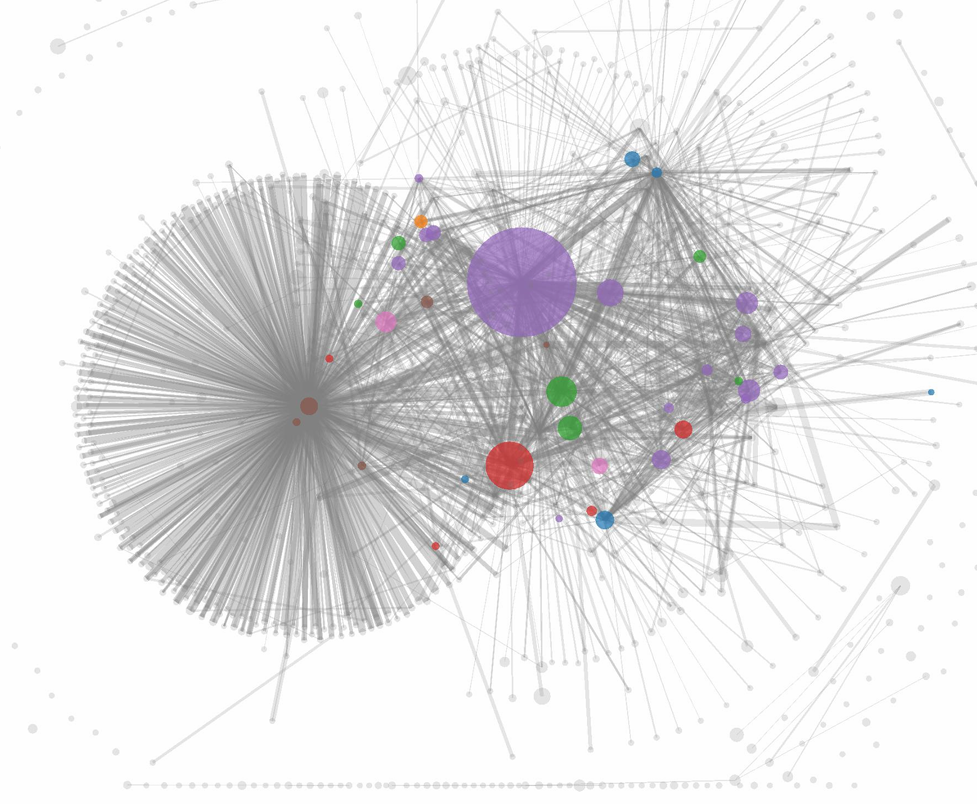
\includegraphics[width=0.6\linewidth]{Images/capitolo_4/grafo_conoscenza.png}
\end{figure}
Possiamo notare che quelli che ricevono tante transazioni sono, in genere, le autorità di cui parlavamo prima. Tra queste, possiamo trovare le più note \textbf{silkroad, satoshi dice, ecc.}.
Siamo a tutti gli effetti riusciti a capire come individuare le grossi autorità ma non è ancora ben chiaro come possiamo a tutti gli effetti deanonimizzare i singoli utenti. Per farlo, l'approccio più semplice è quello del \textit{social engineering}:
\begin{itemize}
    \item \textbf{Transazioni dirette:} Se io faccio in modo che qualcuno mi paghi, trovo il suo indirizzo e, tramite il blockchain explorer, posso vedere quanto si aveva nel portafoglio, da chi ha ricevuto questi soldi ecc.
    \item \textbf{Fornitori di Servizi:} Poiché non tutti possono minare Bitcoin, la maggior parte li compra da servizi esterni come binance e quei servizi devono per leggere conoscere l'identità della persona.
    \item \textbf{Careless:} La gente può deanonimizzarsi da sola pubblicando l'indirizzo online per ricevere donazioni ecc.
    \item \textbf{Attacchi retroattivi:} Poiché vengono scoperte algoritmi sempre più efficaci per raggruppare indirizzi e dato che la blockchain è immutabile, è possibile che in futuro venga scoperto un modo ancora più forte per deanonimizzare qualcuno.
\end{itemize}

\section{De-anonimizzazione a livello Network}
Un altro problema è che pur evitando di pubblicare il proprio indirizzo online, la comunicazione a livello di rete potrebbe fare in modo che qualcuno riesca a deanonimizzarci attraverso l'indirizzo IP. 

Una regola generale è \textit{"Il primo nodo che informa qualcuno di una transazione, è probabile che sia la sua fonte"}. 

\subsection{Rete Tor}
Per evitare questo problema, la soluzione è l'uso della rete \textbf{Tor} un protocollo di rete che si pone come obiettivo quello di garantire l'anonimato a livello di rete.

Quello che vogliamo è una comunicazione di questo tipo:
\begin{itemize}
    \item \textbf{Senders}: Questi invieranno i messaggi all'interno della rete di comunicazione.
    \item \textbf{Communication Network}: Qui arriveranno i messaggi e lì non è ben chiaro il mittente e il destinatario. Questo a patto che questo sistema sia usato da un certo numero di persone poiché altrimenti sarebbe banale il collegamento.
    \item \textbf{Recipients}: Questi riceveranno i messaggi attraverso la rete in maniera del tutto anonima. Cioè, il recipients non saprà nemmeno chi gli ha inviato il messaggio. Per quanto possa sembrare assurdo, questo è appropriato dato che Tor è progettato per la navigazione sul web.
\end{itemize}

Per fare questo, Tor opera secondo un modello di \textbf{cifratura a strati}. Questo sistema è considerato sicuro se \textbf{almeno uno dei router è onesto}. 

Quando Alice deve comunicare con Bob utilizzerà delle chiavi di cifratura valide per la sessione corrente per \textbf{cifrare un messaggio n volte, dove n è il numero di macchine intermedie per cui passa il messaggio}. Ogni macchina intermedia applica una chiave di cifratura per togliere uno strato di cifratura al messaggio fino all’ultima macchina del path prestabilito da Alice. A quel punto il messaggio, ormai in chiaro passa dall’ultima macchina ad Alice.
\begin{figure}[H]
    \centering
    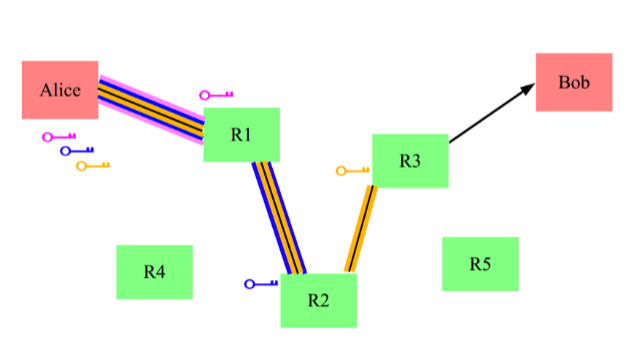
\includegraphics[width=0.7\linewidth]{Images/capitolo_4/cifratura_tor.png}
\end{figure}
Questo sistema è sicuro nel caso in cui ci sia almeno uno nodo onesto. 
Guardiamo i vari casi:
\begin{itemize}
    \item \textbf{Se R2 e R3 sono malevoli}: R1 è onesto e sa da chi viene il messaggio. Tuttavia, poiché onesto questa informazione non verrà trasmessa e, dunque, R2 e R3 possono conoscere B ma non A.
    \item \textbf{Se R1 e R3 sono malevoli}: In questo caso, R2 riceverà l'identità di A inoltrata da R1, tuttavia poiché onesto ignorerà tutte le identità inoltrate e garantirà l'anonimato di A.
    \item \textbf{Se R1 e R2 sono malevoli}: In quest'ultimo caso R3 non invierà comunque le identità ricevute da R2 garantendo l'anonimato di A. 
\end{itemize}
Statisticamente, più server ci sono più il sistema è probabile che sia sicuro poiché è più probabile che ci siano server router onesti. Al tempo stesso, più server ci sono maggiore è la latenza.

\section{Mixing e Anonimato nelle Criptovalute}
Un'idea utile per ottenere anonimato nelle criptovalute è quello di usare degli intermediari che fanno da \textbf{mixing network}.

Questo può essere utilizzato per ottenere anonimato nelle transazioni di criptovalute operando come meccanismo di dissociazione tra indirizzi di input e indirizzi di output per evitare il linking visto precedentemente. L'idea è quella di avere un intermediario per noi a cui mandiamo i messaggi e che poi li manda per noi attraverso dei \textbf{chunk}.

\subsection{Online Wallet}
I wallet online rappresentano una prima forma di mixing, sebbene questo non sia generalmente il loro scopo primario. Questi servizi gestiscono collettivamente i fondi di numerosi utenti, facilitando implicitamente un certo grado di commistione tra i depositi. 

Quando un utente trasferisce Bitcoin a un wallet online e successivamente li preleva, tipicamente riceve unità di valuta diverse da quelle originariamente depositate. Questo processo introduce un elemento di dissociazione che rende più complessa l’analisi della provenienza dei fondi.

Questi, però, presentano diverse limitazioni:
\begin{enumerate}
    \item \textbf{Assenza di garanzie:}  La maggior parte dei wallet online non si impegna formalmente a implementare pratiche di mixing robuste. L’effetto di mixing deriva principalmente da procedure operative interne finalizzate all’ottimizzazione della gestione dei fondi, piuttosto che da un impegno esplicito verso la tutela della privacy degli utenti. 
    \item \textbf{Conservazione dei registri:} Anche ipotizzando un efficace processo di mixing interno, i wallet online generalmente mantengono registri dettagliati delle transazioni effettuate dagli utenti. Questa pratica è adottata sia per ragioni di convenienza operativa, facilitando la risoluzione di controversie e la gestione del servizio, sia per ottemperare a requisiti normativi sempre più stringenti in materia di antiriciclaggio e contrasto al finanziamento del terrorismo.
    \item \textbf{Requisiti di Identificazione:} I wallet online sono sottoposti a regolamentazioni e richiedono la verifica degli utenti.
\end{enumerate}

Quello che vorremmo in realtà sono due caratteristiche fondamentali:
\begin{itemize}
    \item \textbf{Impegno a non conservare registri:} I servizi di mixing dedicati dichiarano esplicitamente di non mantenere archivi delle transazioni processate, eliminando teoricamente la possibilità di ricostruire i collegamenti tra indirizzi di input e output.
    \item \textbf{Assenza di requisiti di Identificazione: } A differenza dei wallet regolamentati, i mixing service non richiedono la verifica dell’identità degli utenti, preservando l’anonimato anche rispetto al provider del servizio stesso
\end{itemize}

\subsection{Principi di Mixing}
Sono stati ideati dei principi fondamentali per ottenere anonimato attraverso sistemi di mixing:
\begin{enumerate}
    \item \textbf{Serie di Mixer}: L'idea è quella di implementare una sequenza di operazioni di mixing successive piuttosto che affidarsi a un singolo intermediario. Questo ha diversi vantaggi:
        \begin{itemize}
            \item \textbf{Riduzione del rischio di compromissione}: L'utilizzo di molteplici mix riduce drasticamente la vulnerabilità del sistema poiché per eliminare l'anonimato bisognerebbe compromettere tutti i mixer contemporaneamente. 
            \item \textbf{Incremento dell'Anonymity set:} Ogni passaggio attraverso un mix diverso espande l’insieme delle transazioni con cui i fondi dell’utente vengono mescolati, aumentando progressivamente la complessità dell’analisi necessaria per deanonimizzare le transazioni.
        \end{itemize}
    \item \textbf{Uniformità delle Transazioni}: Per evitare il link delle transazioni attraverso l'analisi degli importi, è opportuno che i servizi di mixing paghino attraverso transazioni con pagamenti standard detti \textbf{chunk}. Così facendo, poiché tutti spendono/ricevono la stessa quantità di monete in una transazione, non è possibile ricollegare l'origine della moneta alla sua destinazione. Vanno bene anche \textbf{diverse taglie di chunk}.
    \item \textbf{Automatizzazione Lato Client}: Per evitare problemi legati all'elevata complessità della gestione di questo tipo di sistema e, dunque, il possibile errore umano, avrebbe senso far sì che sia lo stesso wallet a gestire questo tipo di meccanismi lato Client in maniera del tutto nascosta al client.
    \item \textbf{Commissioni con All-or-Nothing}: Poiché questo è un servizio di un qualche tipo, è necessario chiaramente pagarlo. Dunque, per garantire l'anonimato anche del servizio stesso, è necessario adottare un meccanismo \textbf{All-or-Nothing} in cui la commissione non è una percentuale della transazione stessa, bensì l'intero importo della transazione che va al servizio con una probabilità ad esempio del $0,01\%$. Questo preserverebbe l'uniformità delle transazioni e proteggerebbe l'anonimato del servizio stesso.
\end{enumerate}
Allo stato attuale delle cose, nessuno adotta realmente questo tipo di mixing per vari motivi tra cui la legge stessa ma anche perché, volendo i servizi lavorare in anonimo, è chiaro che non sarebbe possibile imputarli in alcun modo e, dunque, nessuno avrebbe fiducia in un sistema del genere.

\section{Coinjoin}
Poiché i sistemi di mixing centralizzati hanno dei vincoli imposti dalla centralizzazione stessa, si è cercato di passare a un sistema di \textbf{mixing decentralizzato} così ché non ci sia la necessità di un ente a cui affidarsi e che sia l'utente stesso a gestire i suoi fondi all'interno del processo di mixing.

Qui nasce \textbf{CoinJoin} proposto da \textit{Greg Maxwell}. Questo è un protocollo di mixing decentralizzato che sfrutta una proprietà fondamentale delle transazioni di Bitcoin ossia il sistema di \textbf{firme aggregate} in un'unica transazione. Vedremo nei capitoli successivi i dettagli di questa implementazione. Per fare capire come funziona, l'idea è che per firmare una transazione facciamo in modo che la firma sia generata da tutti coloro che partecipano a questo meccanismo generando firme indipendenti che singolarmente non sono valide ma che aggregate assieme lo sono. 

L'algoritmo procede come segue:
\begin{enumerate}
    \item \textbf{Individuazione dei Peer}: I partecipanti interessati a un round di mixing per un importo specifico devono trovarsi. Comunemente, ciò avviene tramite un server di coordinamento a cui ci si connette, spesso via Tor, per preservare l’anonimato dell’indirizzo IP. I partecipanti si registrano per un round specifico, indicando l’intenzione di mixare un determinato importo, senza ancora rivelare gli UTXO specifici.
    \item \textbf{Fornitura Input/Ouput}: Ogni utente invia al coordinatore l'UTXO che vuole mixare e fornisce una prova di possesso (firma). In questa fase, il coordinatore sa che l'indirizzo $A$ appartiene all'utente 1. L'utente deve fornire l'indirizzo di "uscita" dove riceverà i fondi puliti. 
    Per evitare che il coordinatore colleghi l'input all'output, l'utente invia l'indirizzo di output tramite una nuova connessione Tor e utilizza una firma cieca.
    \item \textbf{Costruzione della Firma}: Il coordinatore invia la transazione completa a tutti i partecipanti.
    Ogni utente controlla la transazione. Firma solo se vede che tra gli output è presente il suo indirizzo con la cifra corretta.
    Se il coordinatore provasse a rubare i soldi o a cambiare un indirizzo, l'utente non firmerebbe e la transazione fallirebbe. Non c'è rischio di furto.
    \item \textbf{Verifica della Firma}: Quando il coordinatore raccoglie le firme di tutti i partecipanti (o della soglia minima richiesta), la transazione diventa valida secondo le regole del protocollo Bitcoin.
    Il coordinatore verifica che tutte le firme siano valide e che la transazione non violi alcuna regola. La transazione viene inviata alla rete Bitcoin. Sulla blockchain apparirà un unico evento in cui 100 persone hanno mescolato i loro soldi, rendendo impossibile per un osservatore esterno sapere chi ha ricevuto cosa.
\end{enumerate}

Questo sistema presenta però alcuni problemi:
\begin{itemize}
    \item \textbf{Individuazione dei Peer}: Un primo ostacolo significativo consiste nell’identificazione di altri utenti interessati al mixing, mantenendo contemporaneamente l’anonimato.
    \item \textbf{Denial of Service}: Partecipanti malevoli potrebbero compromettere l’efficacia del protocollo rifiutandosi di firmare la transazione nelle fasi finali, causando un fallimento del processo di mixing dopo che gli altri utenti hanno già investito tempo e risorse.
\end{itemize}
Per quanto riguarda l'individuazione dei Peer abbiamo già parlato di come le rete Tor sia una soluzione a questo problema creando delle lobby in cui effettuare la ricerca. 
Per quanto riguarda, invece, il Denial of Service, possiamo applicare lo stesso meccanismo che adottiamo su Bitcoin cioè il \textbf{proof of work} o il \textbf{proof of burn}.

